\documentclass{article}
\usepackage{graphicx}
\usepackage[margin=1.5cm]{geometry}
\usepackage{amsmath}

\begin{document}
\twocolumn

\title{Thursday Warm Up, Unit 0: Foundations and Fundamentals}
\author{Prof. Jordan C. Hanson}
\maketitle

\section{Memory Bank}
\small
\begin{itemize}
\item $\cos(2\pi f_1 t) = (1/2) (\exp(2\pi j f_1 t) + \exp(-2\pi j f_1 t))$.
\item $\sin(2\pi f_1 t) = (1/2j) (\exp(2\pi j f_1 t) - \exp(-2\pi j f_1 t))$.
\item $F(f) = \mathcal{F}\left\lbrace f(t)\right\rbrace =\int_{-\infty}^{\infty} f(t) e^{-2\pi jft} dt$ ... The Fourier Transform.
\item $\mathcal{F}^{-1}\left\lbrace F(f)\right\rbrace =\int_{-\infty}^{\infty} F(f) e^{2\pi jft} df$ ... The Inverse Fourier Transform.
\item \textbf{Convolution}: this is an operation that characterizes the response $h[n]$ of a linear system.
\begin{equation}
y[i] = h[n] * x[n] = \sum_{j=0}^{M-1}h[j]x[i-j] \label{eq:conv}
\end{equation}
In words, the output at sample $i$ is equal to the produce of the system response $h$ and the input signal $x$, summed over the proceeding $M$ samples (from $j=0$ to $j=M-1$).
\end{itemize}

\section{Interpreting Spectra: amplitude modulation (AM)}

\begin{enumerate}
\item Consider Fig. \ref{fig:1} (top). In this exercise, we will develop an understanding of \textbf{amplitude modulation.} (a) Express the following functions as complex exponentials: $A\cos(2\pi f_1 t)$ and $(m/A)\cos(2\pi f_2 t)$. (b) Multiply the two functions, and show that the result is a pair of sinusoids at two new frequencies.  What are the new frequencies? (c) Sketch what you think the Fourier spectrum would be, and compare it to Fig. \ref{fig:1} (bottom).  Fig. \ref{fig:2} contains an LC resonator circuit, which retains the carrier frequency in the spectrum. \\ \vspace{5cm}
\end{enumerate}

\section{Convolution and Impulse Response}

\begin{enumerate}
\item Notice the definition of \textbf{convolution}, Eq. \ref{eq:conv}. Let $x[n]$ be the input signal, $h[n]$ be the response of a linear DSP system, and $y[n]$ be the output signal. (a) Show that $y[n] = h[n]$, if $x[n] = \delta[n]$. (b) What is $y[n]$, if $x[n] = [0000 1000]$, and $h[n] = [\frac{1}{2} \frac{1}{2} 000000]$? (c) Using the \verb+conv+ function in \verb+octave+, write a short code that produces the result of the convolution in (b).
\end{enumerate}

\begin{figure}
\centering
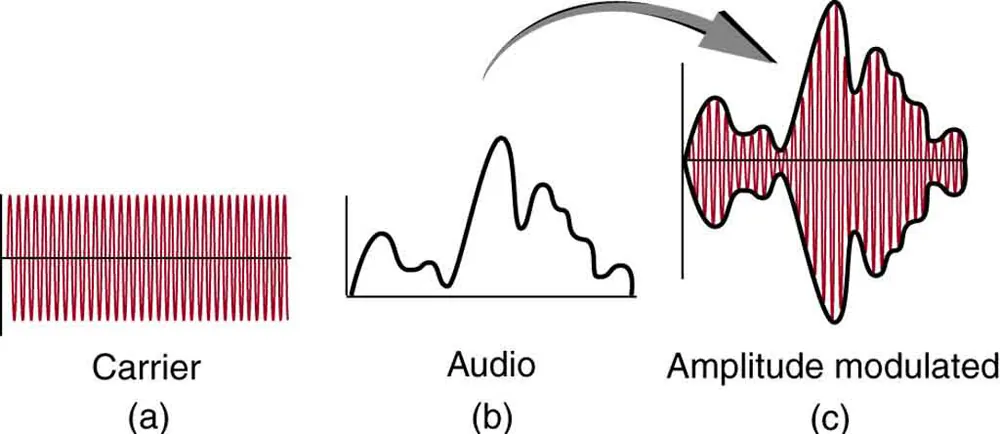
\includegraphics[width=0.33\textwidth]{AM.png} \\
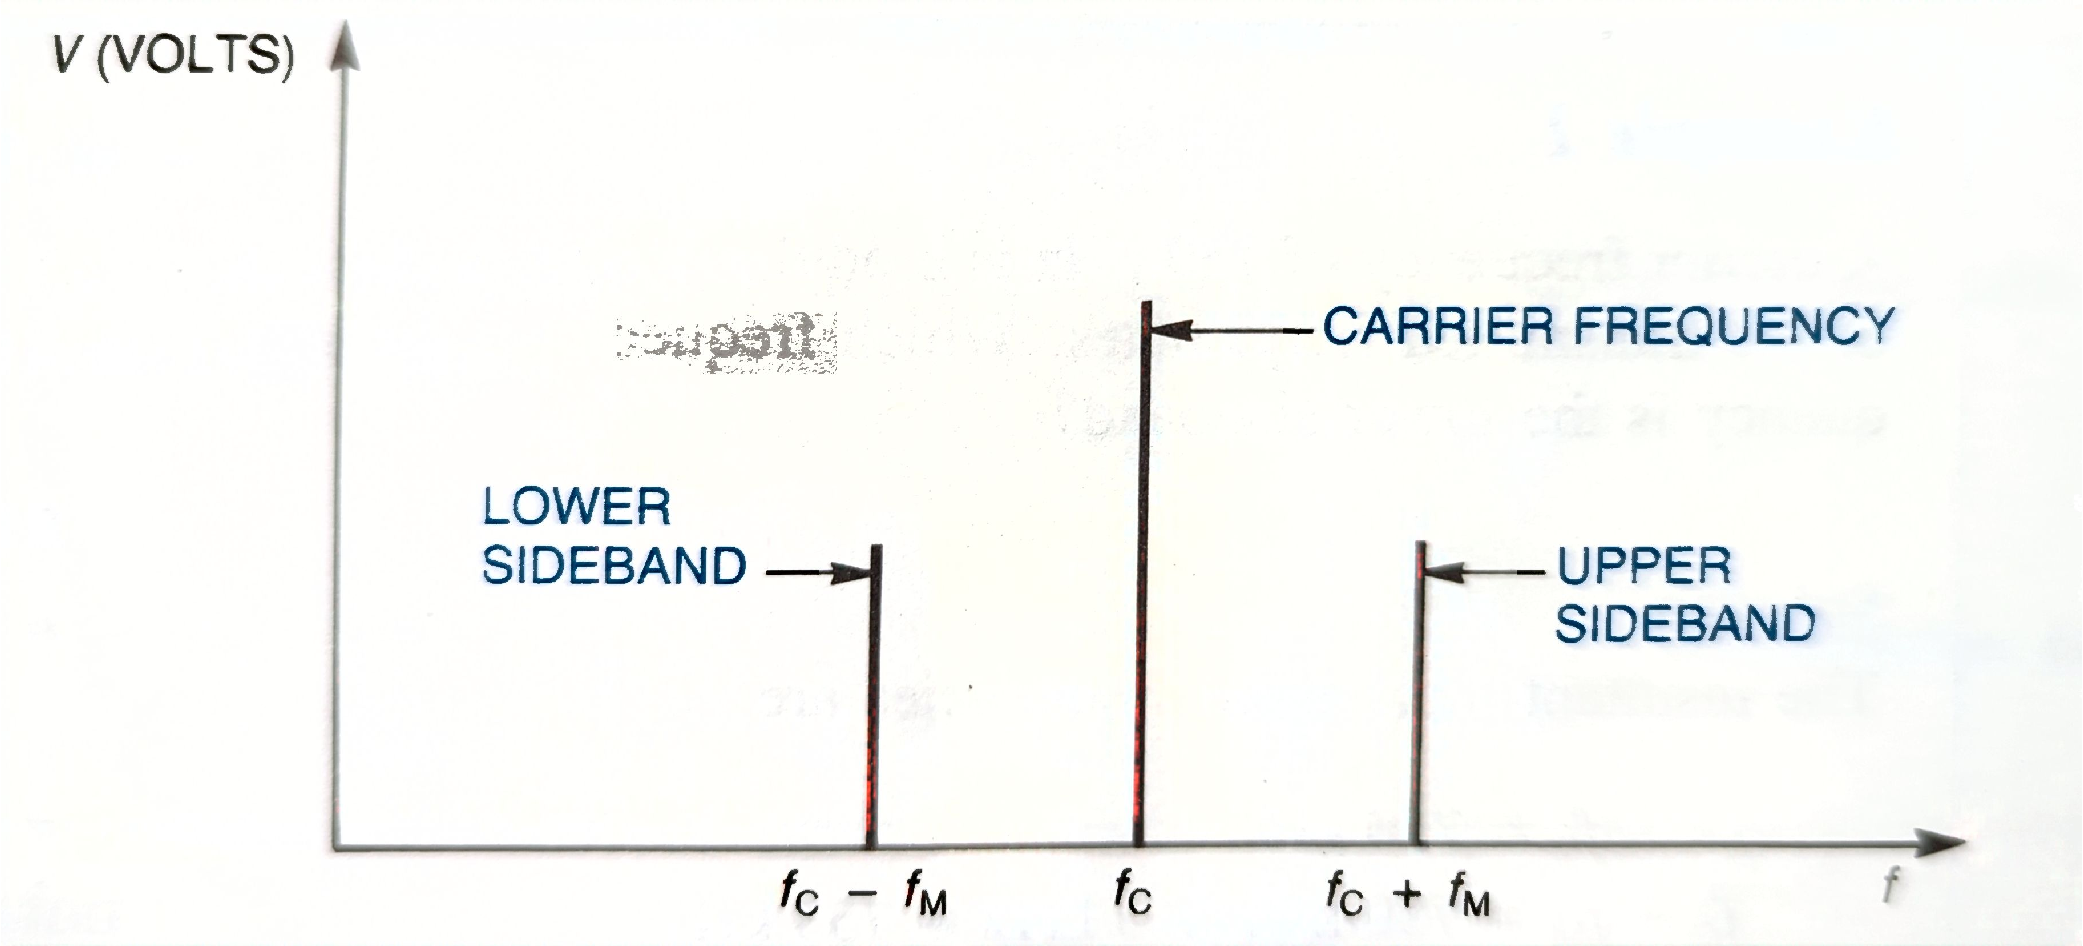
\includegraphics[width=0.45\textwidth]{AMSpec.pdf}
\caption{\label{fig:1} Amplitude modulation signal and spectrum.}
\end{figure}

\begin{figure}
\centering
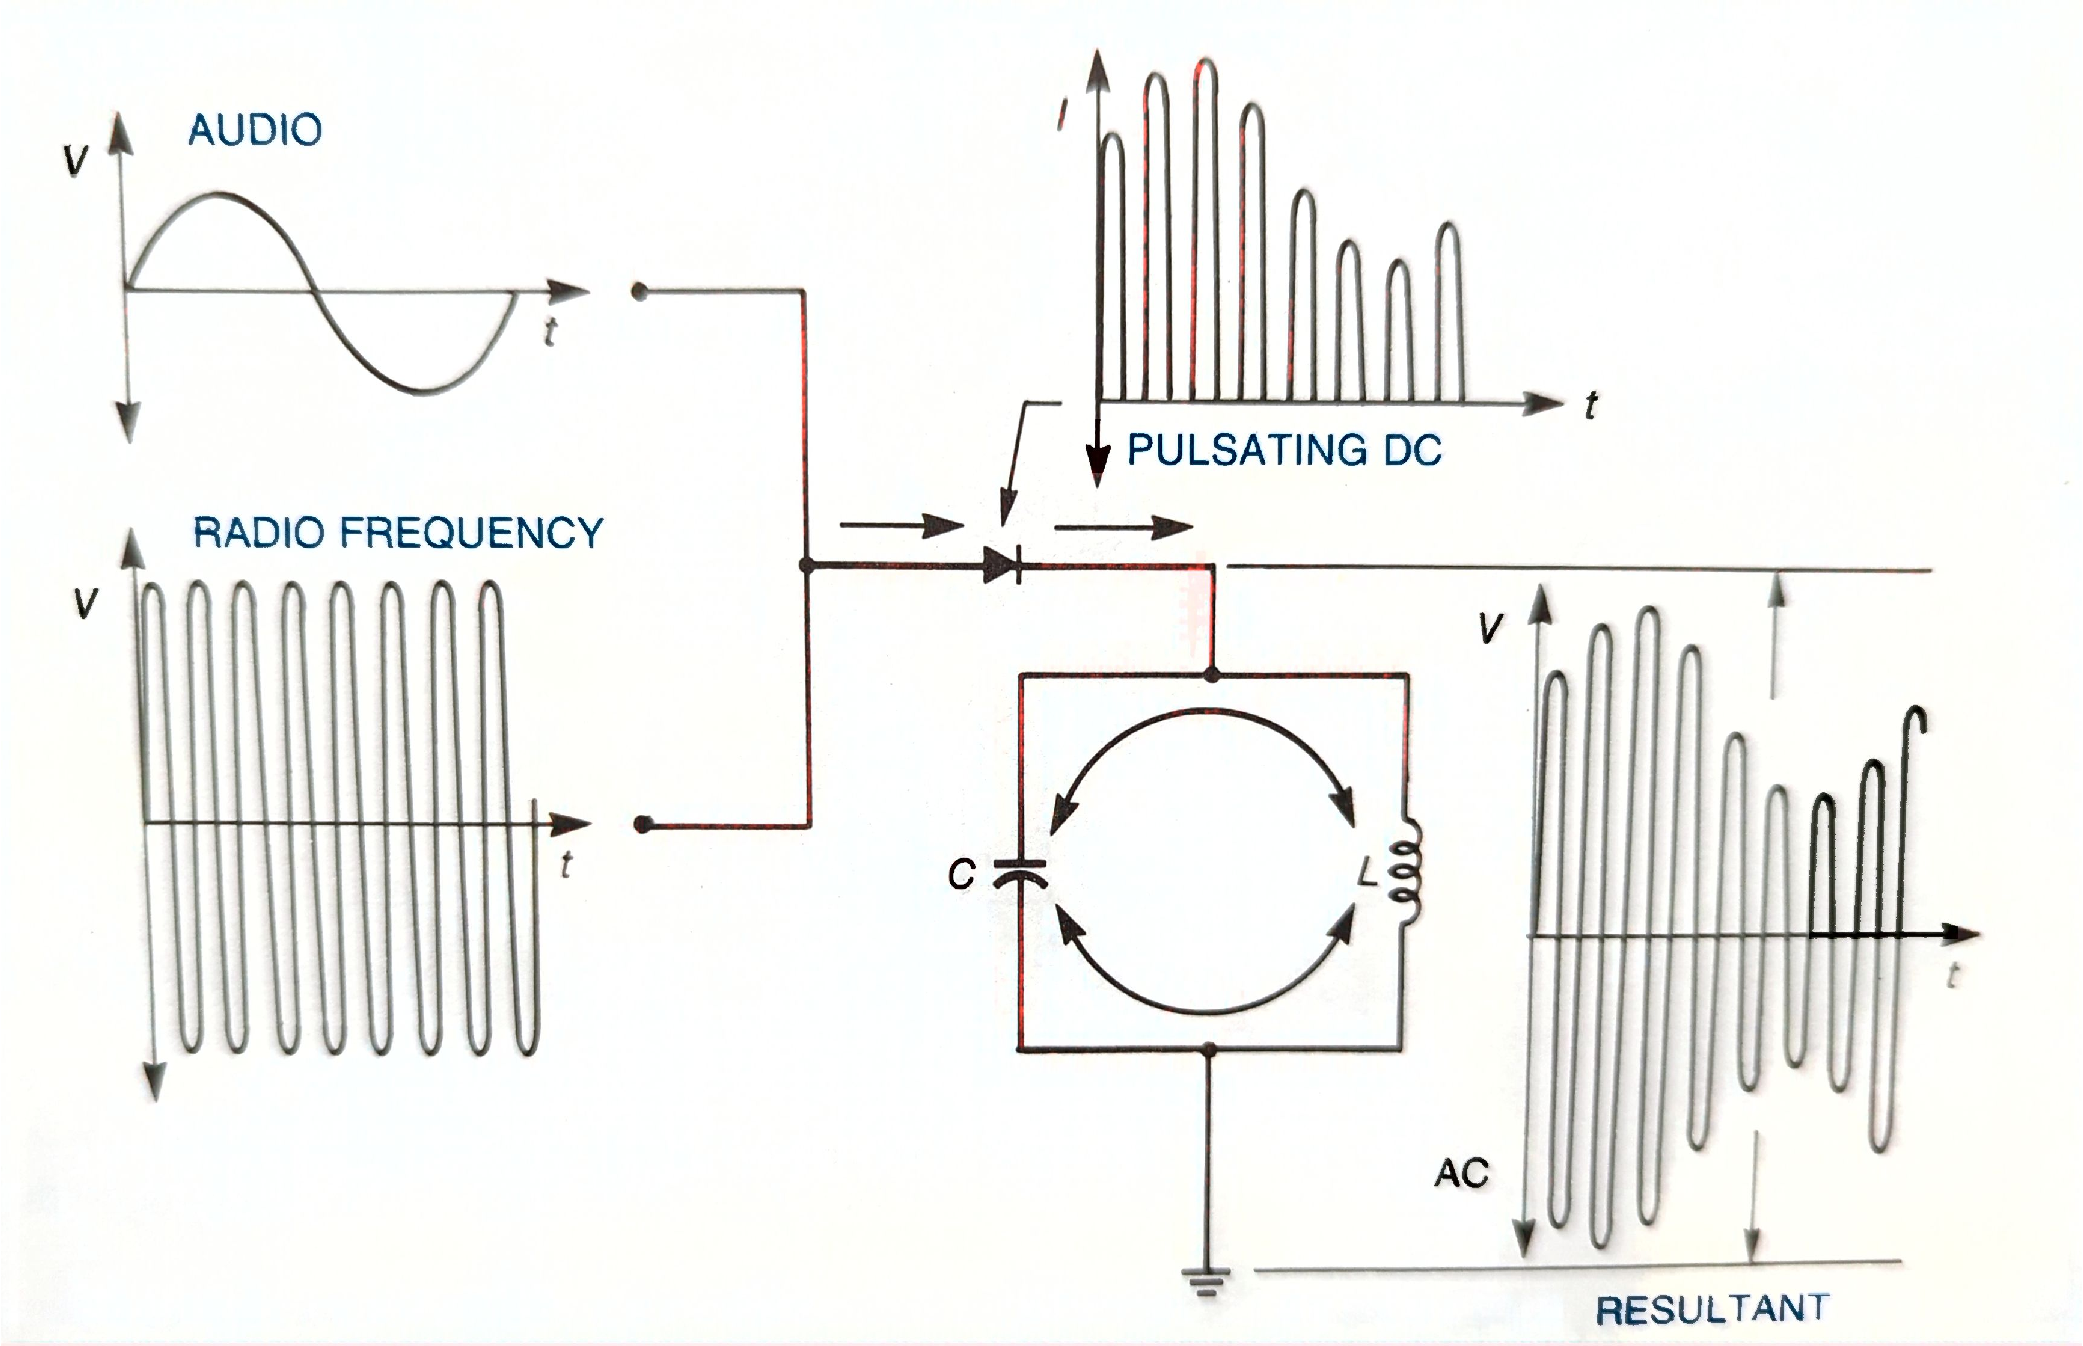
\includegraphics[width=0.4\textwidth]{AMSpec3.pdf}
\caption{\label{fig:2} Amplitude modulation circuit.}
\end{figure}

\end{document}
